% page format, etc.
\documentclass[pdftex, a4paper, oneside, parskip, numbers=noenddot, listof=totoc, bibliography=totocnumbered, hyperfootnotes=false]{scrreprt}

\newcommand{\thesistitle}{Natürlichsprachliche Mustererkennung für natürlichsprachliche Objektszenarien}
\newcommand{\thesistype}{B A C H E L O R A R B E I T}
\newcommand{\thesistypedesc}{im Fachbereich Elektrotechnik/Informatik \\
der Universität Kassel}
\newcommand{\thesisauthorname}{Adrian Kunz}
\newcommand{\thesisauthorhomestreet}{***REMOVED***}
\newcommand{\thesisauthorhometown}{36199 Rotenburg a.d. Fulda}
\newcommand{\thesisauthormatrikelnumber}{35013235}
\newcommand{\thesisauthoremail}{***REMOVED***}
\newcommand{\thesisdepartment}{Fachgebiet Software Engineering}
\newcommand{\thesisfirstreviewer}{Prof. Dr. Albert Zündorf}
\newcommand{\thesissecondreviewer}{Prof. Dr. Claude Draude}
\newcommand{\thesissupervisor}{Prof. Dr. Albert Zündorf}
\newcommand{\thesisdate}{31. März 2020}

% geometry
\usepackage[bindingoffset=1cm, left=2.5cm, right=2.5cm, top=2.5cm, bottom=2.5cm]{geometry}

% Headline
\usepackage{fancyhdr}
\pagestyle{fancy}
\renewcommand{\chaptermark}[1]{\markboth{\thechapter\ #1}{}}
\lhead{\leftmark} \rhead{\thepage}
\cfoot{}
\fancypagestyle{plain}{}

% Select input encodung, usually utf8 is the best choice, on windows, \usepackage[latin1]{inputenc} maybe required
\usepackage[utf8]{inputenc}
\usepackage[T1]{fontenc}

% Colors
\usepackage{color}
\usepackage{colortbl}

% Tables
\usepackage{tabularx}
\usepackage{multirow}

% Drawing graphs etc.
\usepackage{pgf}
\usepackage{tikz}
\usetikzlibrary{arrows,automata}

% math
\usepackage{amsmath}

% lists
\usepackage{paralist}

% Figures
\usepackage{graphicx, wrapfig}

% Hyperlinks
\usepackage[hyphens]{url}
\usepackage{hyperref}
\hypersetup{colorlinks, citecolor=black, linkcolor=black, urlcolor=black}

% Minted
\usepackage[chapter]{minted}
%\usemintedstyle{xcode}
\setminted{frame=single,tabsize=2,linenos}

\newmintinline[code]{text}{breaklines}
\newmintinline[mdcode]{md}{breaklines}
\newmintinline[jcode]{java}{breaklines}

\newminted[codeblock]{text}{autogobble,frame=none,linenos=false,breaklines}
\newminted[mdcodeblock]{md}{autogobble,frame=none,linenos=false,breaklines}
\newminted[jcodeblock]{java}{autogobble,frame=none,linenos=false}

\newcommand{\outquote}[1]{``{#1}''}

\newcommand{\codelisting}[4]{%
    \begin{listing}[htp]
        \inputminted{#1}{#2/#3}
        \vspace{-3ex}
        \caption{#4}
        \label{lst:#3}
    \end{listing}%
}

% list of abbreviations
\usepackage[printonlyused]{acronym}

% Set line pitch
\usepackage{setspace}
\onehalfspacing              % anderthalbzeilig (oder auch \doublespace)

% Newcommand TODO (red in text)
\newcommand{\todo}[1]{\textcolor{red}{TODO: #1}}

% Newcommand TODOM (red at border)
\newcommand{\todom}[1]{\marginpar{\parbox{1.5cm}{\textcolor{red}{TODO:\\ #1}}}}

%fancyBox
%\usepackage{fancybox}

% Layout corrections (Schusterjungen)
\clubpenalty = 10000
% Layout corrections (Hurenkinder) 
\widowpenalty = 10000
\displaywidowpenalty = 10000

% Figures
\usepackage{caption}
\usepackage[hypcap=true,labelformat=simple]{subcaption}
\renewcommand{\thesubfigure}{(\alph{subfigure})}

% Tables
\usepackage{booktabs}

% Frequently used column types
\newcolumntype{C}[1]{>{\centering\arraybackslash}p{#1}} % centering column type with fixed width
\newcolumntype{R}[1]{>{\raggedleft\arraybackslash}p{#1}} % right aligned column type with fixed width
\newcolumntype{L}[1]{>{\raggedright\arraybackslash}p{#1}} % left aligned column type with fixed width

% Shortcuts for referencing floats:
\newcommand{\fig}[1]{\figurename~\ref{#1}} %shortcut for a figure reference
\newcommand{\tab}[1]{Table~\ref{#1}} %shortcut for a table reference
\newcommand{\eq}[1]{(\ref{#1})} %shortcut for an equation reference
\newcommand{\lst}[1]{Listing~\ref{#1}} %shortcut for a listing reference
\newcommand{\sect}[1]{Section~\ref{#1}} %shortcut for a Section reference


\usepackage[ngerman]{babel}

\begin{document}

% use small roman page numbering
\pagenumbering{roman}

\begin{titlepage}
	%select font without serifs
	\sffamily

	% Logo
	\begin{tabularx}{\textwidth}{@{}l@{}>{\raggedleft\arraybackslash}X@{}r@{}}
		\multirow{2}{*}{
\includegraphics[width=6.8cm]{images/Logo_UniKassel}} &
		\raisebox{-1mm}{\small{Fachbereich Elektrotechnik/Informatik}} \\
		&\raisebox{-1mm}{\small{Fachgebiet Digitaltechnik}} &
	\end{tabularx}

	\vspace{2.5cm}

	\begin{center}
		% Title and subtitle
		\huge{\thesistitle}

		\vspace{3cm}

		\renewcommand{\baselinestretch}{1.3}
		\Large{\thesistype}

		\large
		\thesistypedesc
	\end{center}

	\vspace{1.5cm}
	\renewcommand{\baselinestretch}{1}
	\begin{table}[htpb]
		\centering
		\begin{tabular}{ll}
			\\
			Eingereicht von: & \thesisauthorname \\
			Anschrift: & \thesisauthorhomestreet \\
			& \thesisauthorhometown \\
			\\
			Matrikelnummer: & \thesisauthormatrikelnumber \\
			Emailadresse: & \thesisauthoremail \\
			\\
			Vorgelegt im: & \thesisdepartment \\
			\\
			Gutachter: & \thesisfirstreviewer \\
			& \thesissecondreviewer \\
			\\
			Betreuer: & \thesissupervisor \\
			\\
			eingereicht am: & \thesisdate \\
		\end{tabular}
	\end{table}

	% font with serifs
	\rmfamily
\end{titlepage}

\chapter*{Zusammenfassung}

% Inhaltsverzeichnis und Kopfzeile
\addcontentsline{toc}{chapter}{Zusammenfassung}
\markboth{Zusammenfassung}{Zusammenfassung}

Diese Arbeit führt eine neue Online-Plattform für elektronische Lehre ein, die thematisch auf Datenmodellierung fokussiert ist.
Dafür wird eine neue Beschreibungssprache vorgestellt, die die Modellierung anhang von textuellen Beispielszenarien in natürlicher Sprache ermöglicht.
Auf der Online-Plattform ist das Einreichen von Aufgaben und Lösungen möglich, wovon letztere automatisch korrigiert werden können.
Dies wird durch Funktionalität zur Mustererkennung auf beliebigen Objektstrukturen in der Sprache der Beispielszenarien realisiert.

%%%%%%%%%%%%%%%%%%%%%%%%%%%%%%%%%%%%%%%%%%%%%%%%%%%%%%%%%%%%%%%%%%%%%%%%%%%%%
\chapter*{Erklärung}
%%%%%%%%%%%%%%%%%%%%%%%%%%%%%%%%%%%%%%%%%%%%%%%%%%%%%%%%%%%%%%%%%%%%%%%%%%%%%

%%%%%%%%%%%%%%%%%%%%%%%%%%%%%%%%%%%%%%%%%%%%%%%%%%%%%%%%%%%%%%%%%%%%%%%%%%%%%
% Inhaltsverzeichnis und Kopfzeile
\addcontentsline{toc}{chapter}{Erklärung}
\markboth{Erklärung}{Erklärung}
%%%%%%%%%%%%%%%%%%%%%%%%%%%%%%%%%%%%%%%%%%%%%%%%%%%%%%%%%%%%%%%%%%%%%%%%%%%%%
Hiermit erkläre ich, dass ich die vorliegende Arbeit selbstständig und nur mit den nach der Prüfungsordnung der Universität Kassel zulässigen Hilfsmitteln angefertigt habe.
Die verwendete Literatur ist im Literaturverzeichnis angegeben.
Wörtlich oder sinngemäß übernommene Inhalte habe ich als solche kenntlich gemacht.\\

\vspace{1cm}

Kassel, 31.03.2020

\begin{flushright}
  \underline{\hspace{7cm}} \\
  Adrian Kunz
\end{flushright}

%%%%%%%%%%%%%%%%%%%%%%%%%%%%%%%%%%%%%%%%%%%%%%%%%%%%%%%%%%%%%%%%%%%%%%%%%%%%%%
\chapter*{Declaration}
%%%%%%%%%%%%%%%%%%%%%%%%%%%%%%%%%%%%%%%%%%%%%%%%%%%%%%%%%%%%%%%%%%%%%%%%%%%%%

%%%%%%%%%%%%%%%%%%%%%%%%%%%%%%%%%%%%%%%%%%%%%%%%%%%%%%%%%%%%%%%%%%%%%%%%%%%%%
% Inhaltsverzeichnis und Kopfzeile
\addcontentsline{toc}{chapter}{Declaration}
\markboth{Declaration}{Declaration}
%%%%%%%%%%%%%%%%%%%%%%%%%%%%%%%%%%%%%%%%%%%%%%%%%%%%%%%%%%%%%%%%%%%%%%%%%%%%%
Herewith I declare, that I have made the presented paper myself and solely
with the aid of the means permitted by the examination regulations of the
University of Kassel.
The literature used is indicated in the bibliography.
I have indicated literally or correspondingly assumed contents as such.

\vspace{1cm}

Kassel, 31.03.2020

\begin{flushright}
  \underline{\hspace{7cm}} \\
  Adrian Kunz
\end{flushright}


% TOC, list of figures, list of listings, etc. (use what is appropriate)
\addtocontents{toc}{\protect\vspace{0.2cm}}
\tableofcontents
\listoffigures
\listoftables
\lstlistoflistings

% arabic page numbering
\pagebreak
\pagenumbering{arabic}
\addtocontents{toc}{\protect\vspace{1.0cm}}

\chapter{Einleitung / Introduction}

Some guidelines and examples are given in the following.

\section{Citations}

Citations should be made using BibTeX in the file \verb|thesis.bib|.
Using BibTeX, different styles are available for different types of publications. Examples are books \cite{Adams90}, journal articles \cite{Zhang99}, conference proceeding \cite{Yee99} and
electronic resources \cite{Fear05}. Multiple references can be made by \cite{Adams90,Zhang99,Yee99,Fear05}.


\section{Figures}

A simple example of a figure can be found in \fig{fig:simple_figure}. A more complex figure including subfigures is show in \fig{fig:figure_with_subfigures}. Here each subfigure can be addressed separately (e.g., \fig{fig:subfigure1} and \fig{fig:subfigure2}). Please use vector graphics (pdf, eps obtained from svg, etc.) whenever possible. Pixel formats like jpeg, bmp, etc. should only be used for real photographs.

\begin{figure}[!h]
	\centering
	\fbox{\parbox{5cm}{\centering ~\vspace{1.5cm}\\Dummy\\~\vspace{1.5cm}}} %replace this line by: \includegraphics{path to image}
	\caption{Simple figure}
	\label{fig:simple_figure}
\end{figure}

\begin{figure}[!h]
	\centering
	\begin{subfigure}[b]{7cm}
		\centering
		\fbox{\parbox{5cm}{\centering ~\vspace{1.5cm}\\Dummy\\~\vspace{1.5cm}}} %replace this line by: \includegraphics{path to image}
		\caption{Caption of subfigure a (can be empty)}
		\label{fig:subfigure1}
	\end{subfigure}
	\begin{subfigure}[b]{7cm}
		\centering
		\fbox{\parbox{5cm}{\centering ~\vspace{1.5cm}\\Dummy\\~\vspace{1.5cm}}} %replace this line by: \includegraphics{path to image}
		\caption{Caption of subfigure b (can be empty)}
		\label{fig:subfigure2}
	\end{subfigure}
	\caption{Figure using subfigures}
	\label{fig:figure_with_subfigures}
\end{figure}


\section{Tables}

Examples of tables can be found in \tab{tab:simple_table} and \tab{tab:complex_table}. In general vertical lines are not necessary and should be avoided (see \cite{Fear05} for more about table styles).

\begin{table}[!h]
	\renewcommand{\arraystretch}{1.1}
	\caption{A very simple table}
	\label{tab:simple_table}
	\centering
	\begin{tabular}{cccc}
		\toprule
		& Apple & Orange & Banana \\
		\midrule
		Colour       & green & orange & yellow\\
		\bottomrule
	\end{tabular}
\end{table}

\begin{table}[!h]
	\renewcommand{\arraystretch}{1.1}
	\caption{An example of a more complex table}
	\label{tab:complex_table}
	\centering
	\begin{tabular}{ccC{1cm}C{1cm}C{1cm}C{1cm}C{1cm}C{1cm}C{1cm}C{1cm}C{1cm}C{1cm}C{1cm}}
		\toprule
		& & \multicolumn{4}{c}{RPAG algorithm} & \multicolumn{5}{c}{RPAGT (proposed)}\\
		\cmidrule(rl){3-6} \cmidrule(rl){7-11}
		$N$ & $N_\text{uq}$ & S & add ops & pure reg. & reg. ops & S & add ops & pure reg. & reg. ops & impr.\\
		\cmidrule(rl){1-11}
		6   & 3  & 3 & 8  & 1 & 9  & 2 & 5  & 0 & 5  & 44.4\% \\
		10  & 5  & 3 & 10 & 3 & 13 & 2 & 6  & 2 & 8  & 38.5\% \\
		13  & 7  & 3 & 14 & 2 & 16 & 2 & 8  & 2 & 10 & 37.5\% \\
		20  & 10 & 3 & 15 & 4 & 18 & 2 & 9  & 3 & 12 & 33.3\% \\
		28  & 14 & 3 & 20 & 3 & 23 & 2 & 15 & 2 & 17 & 26.1\% \\
		41  & 21 & 3 & 31 & 1 & 32 & 2 & 23 & 2 & 25 & 21.9\% \\
		61  & 31 & 3 & 39 & 3 & 42 & 2 & 32 & 2 & 34 & 19.0\% \\
		119 & 54 & 3 & 62 & 7 & 69 & 2 & 56 & 1 & 57 & 17.4\% \\
		151 & 71 & 3 & 79 & 4 & 83 & 2 & 72 & 2 & 74 & 10.8\% \\
		\cmidrule(rl){1-11}
		avg.: & 24 & & 30.89 & 3.56 & 33.89 & & 25.11 & 1.78 & 26.89 & 27.7\% \\
		\bottomrule
	\end{tabular}
\end{table}

\section{Listings}

Listings can be included in the text using the \verb|lstlisting| environment. An example listing is shown in \lst{lst:pseudocode}. The listing format is set for pseudocodes (based on the C language). For other languages adjust the settings in \verb|header.tex|.

\begin{lstlisting}[float,caption=RPAGT Algorithm,label=lst:pseudocode]
	RPAGT($T$)
	$\displaystyle S := \max_{t\in T} \, \text{AD}_{\text{min}}^3(t)$
	$X_S := \{\text{odd}(t) \ | \ t \in T\} \setminus \{0\}$
	for $s=S\ldots 2$
	$W := X_s$
	$P := \emptyset$
	do
	$p \leftarrow \text{best\_single\_predecessor}(P,W,s)$
	if $p \neq 0$
	$P \leftarrow P \cup \{p\}$
	else
	$P' \leftarrow \text{best\_msd\_predecessor\_set}(W,s)$
	$P \leftarrow P \cup P'$
	$W \leftarrow W \setminus \mathcal{A}^3_{*}(P)$
	while $|W|\neq \emptyset$
	$X_{s-1} \leftarrow P$
\end{lstlisting}

\section{ToDo's}

During the writing of the thesis, ToDo's in the text can be highlighted using \verb|\todo|. Notes at the border of the text can be done using \verb|\todom|.
\todo{This has to be more extended}
\todom{ToDo remark at the border}


\begin{appendix}
	\chapter{Anhang}\label{ch:appendix}

\section{Vollständiger Java-Code für UserRegistry-Beispiel}\label{sec:user-registry-full}

\begin{center}
    \code{User.java}
    \inputminted[breaklines]{java}{chapter/fulib-scenarios/java/User.java}

    \code{UserRegistry.java}
    \inputminted[breaklines]{java}{chapter/fulib-scenarios/java/UserRegistry.java}

    \code{UserRegistryTest.java}
    \inputminted[breaklines]{java}{chapter/fulib-scenarios/java/UserRegistryTest.java}
\end{center}

\section{Scenario-Lexer-Grammatik}\label{sec:scenario-lexer-grammar}

\inputminted[breaklines]{antlr}{chapter/fulib-scenarios/grammars/ScenarioLexer.g4}

\section{Scenario-Parser-Grammatik}\label{sec:scenario-parser-grammar}

\inputminted[breaklines]{antlr}{chapter/fulib-scenarios/grammars/ScenarioParser.g4}

\section{GenTreeSrc-Definitionsdatei}\label{sec:gts-definitions}

\inputminted[breaklines]{java}{chapter/fulib-scenarios/definitions/FulibScenarios.gts}

\section{Ergebnisse der Vorlesungsumfrage PM 19/20 zu fulib.org, FulibScenarios und FulibMockups}\label{sec:survey-results}

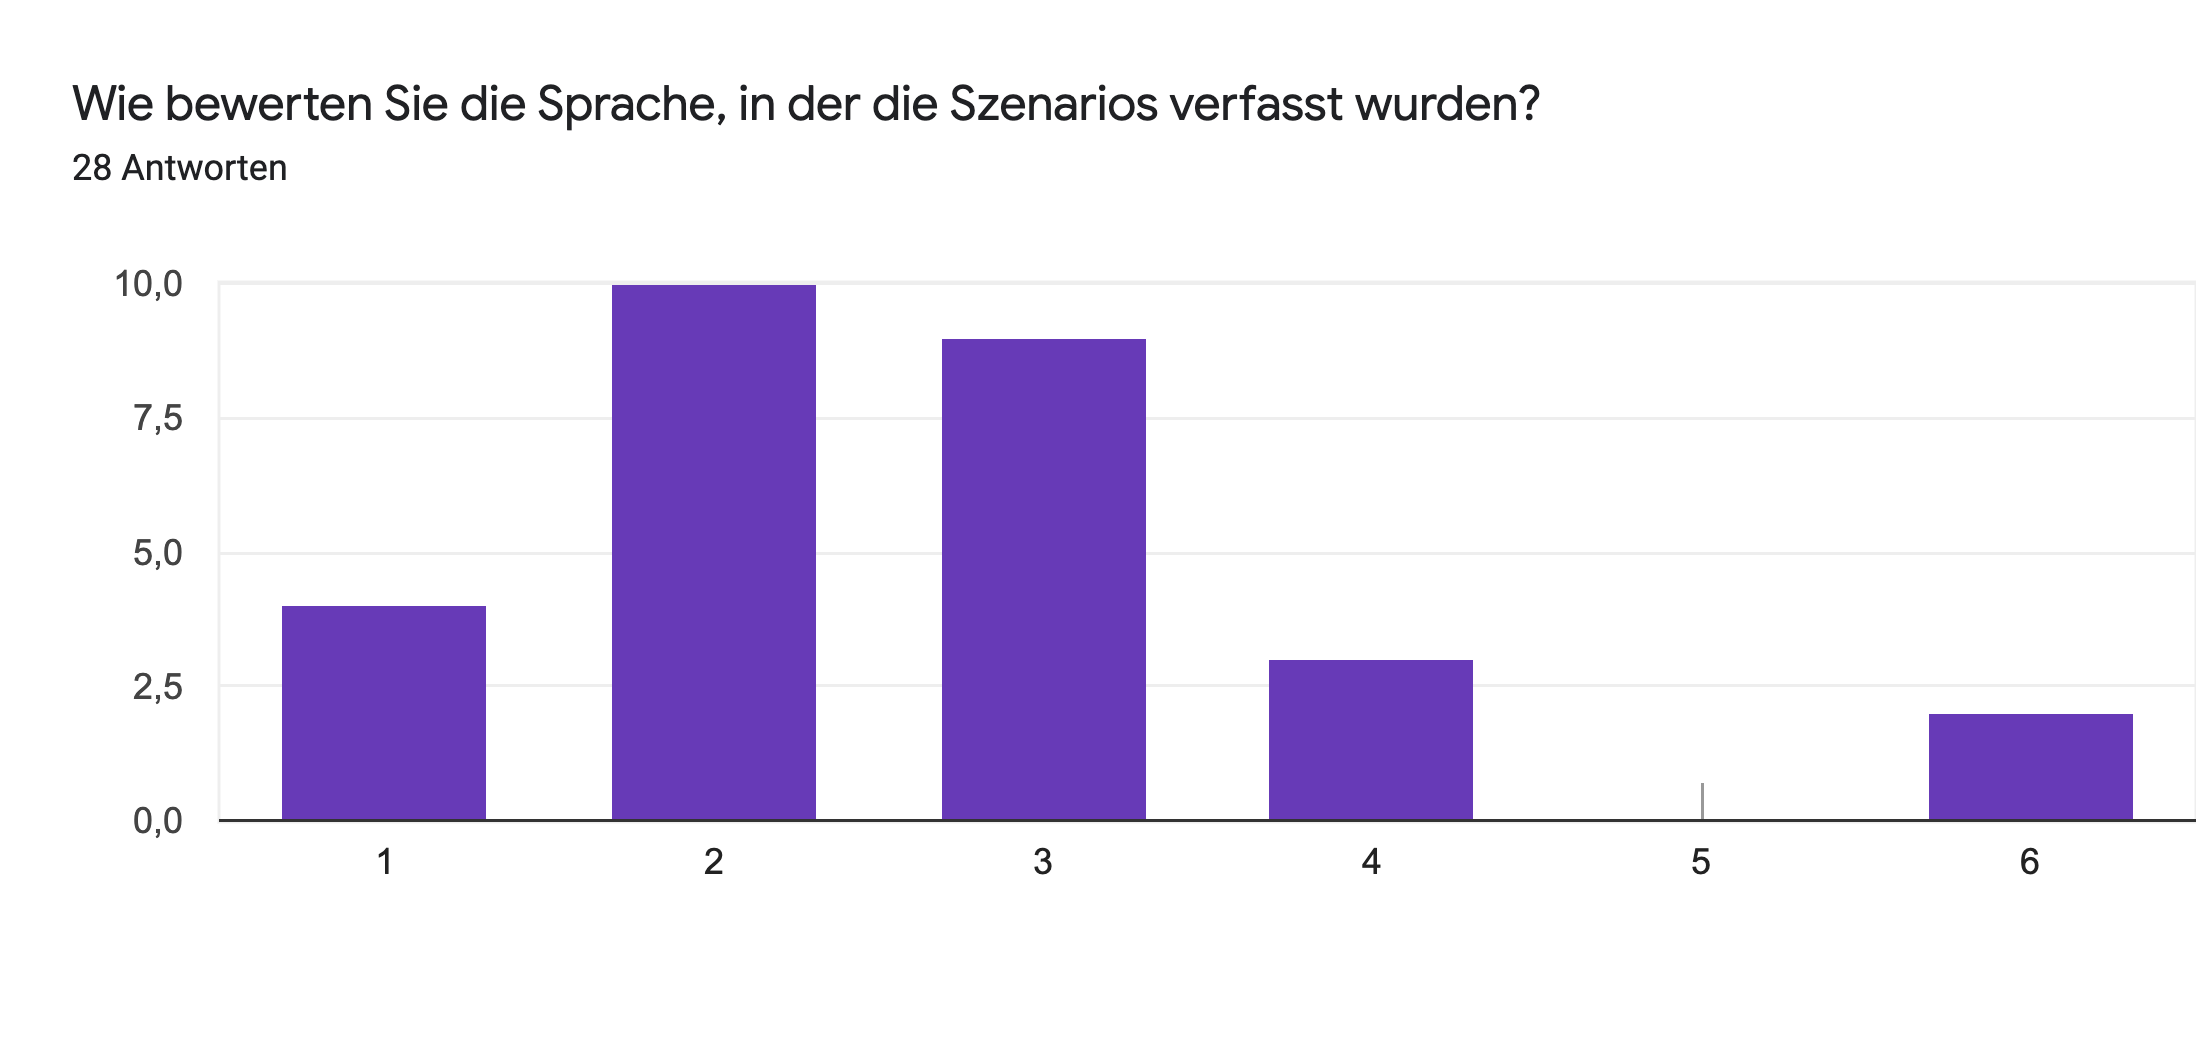
\includegraphics[width=\textwidth]{images/language.png}
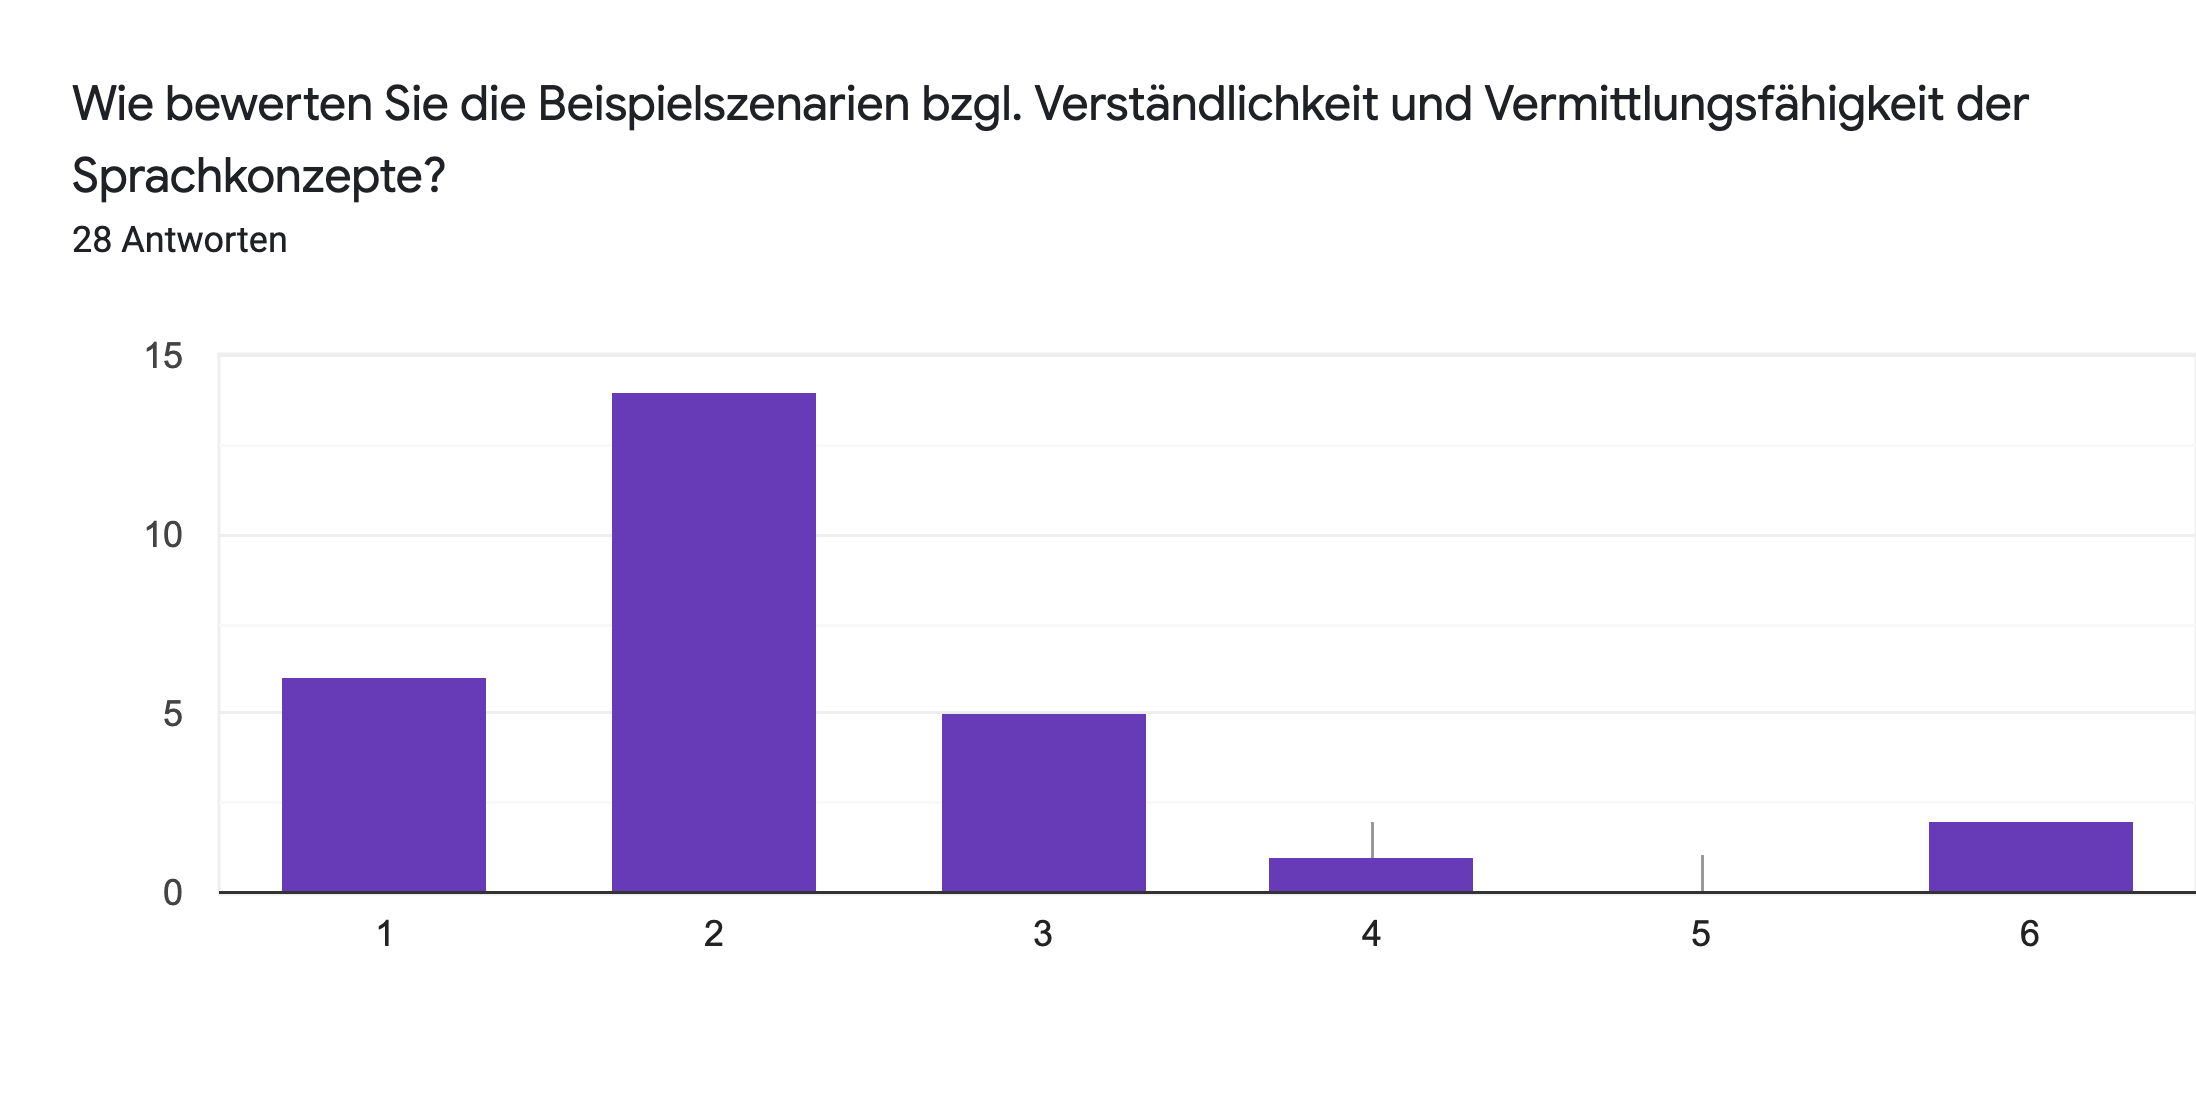
\includegraphics[width=\textwidth]{images/examples.png}
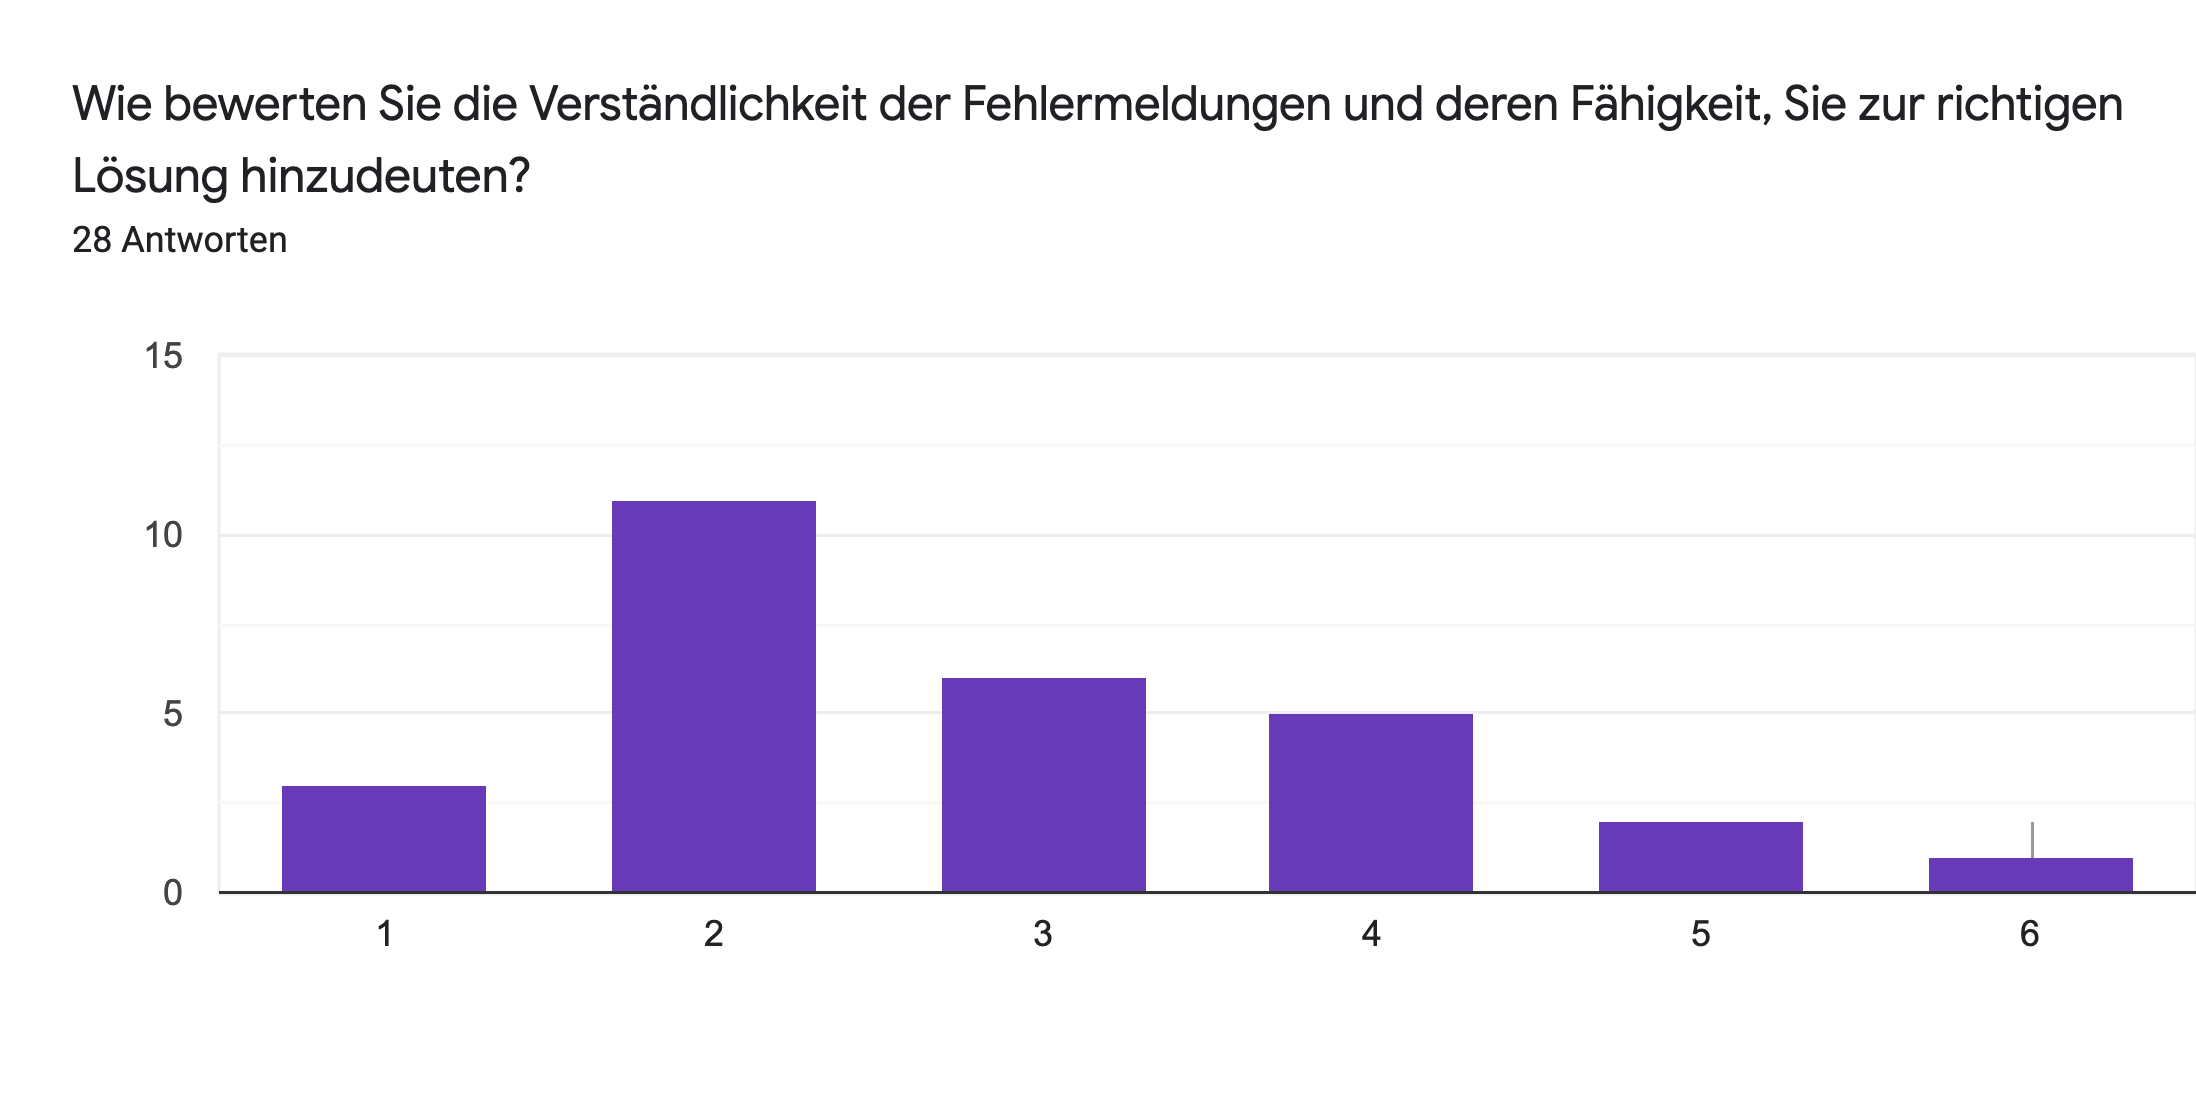
\includegraphics[width=\textwidth]{images/errors.png}
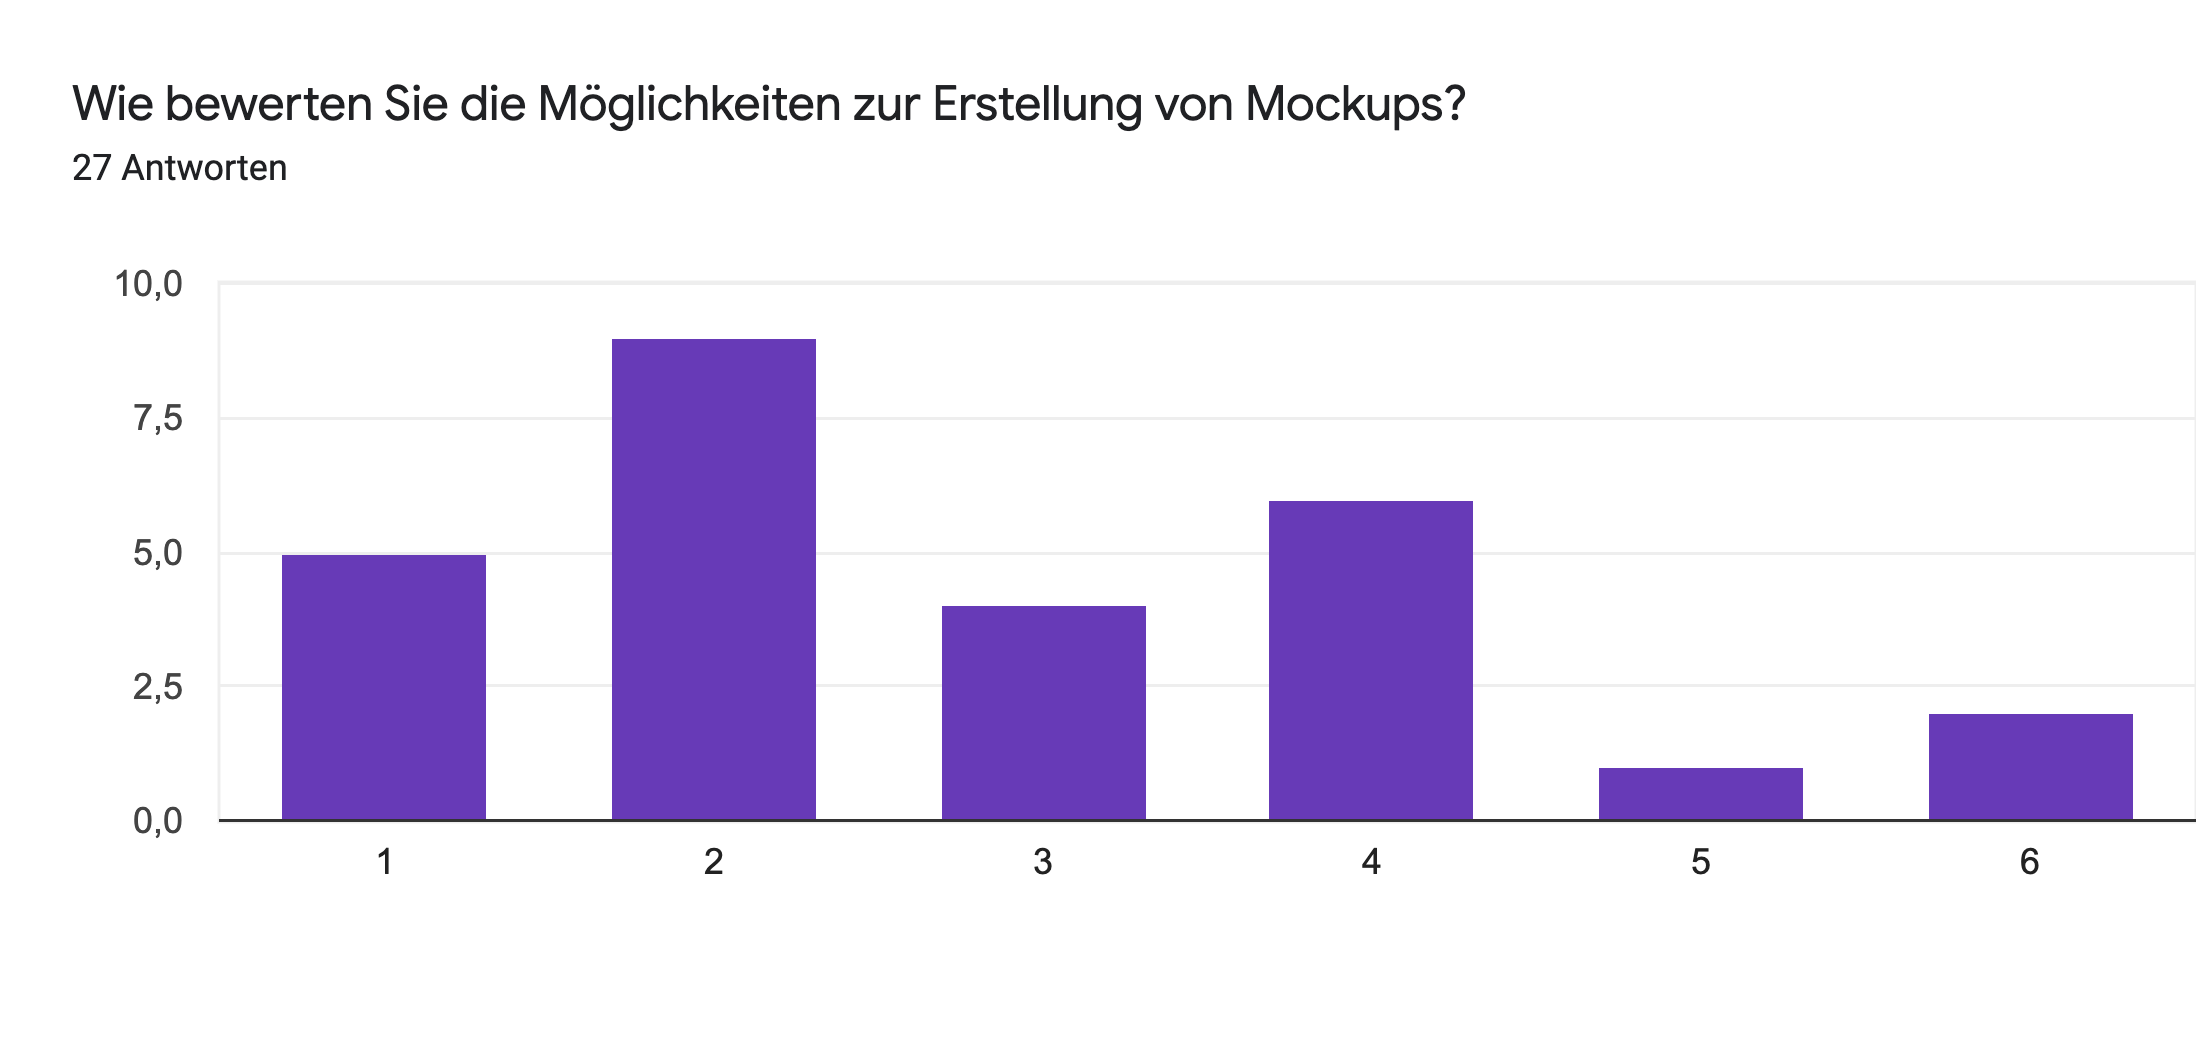
\includegraphics[width=\textwidth]{images/mockups.png}
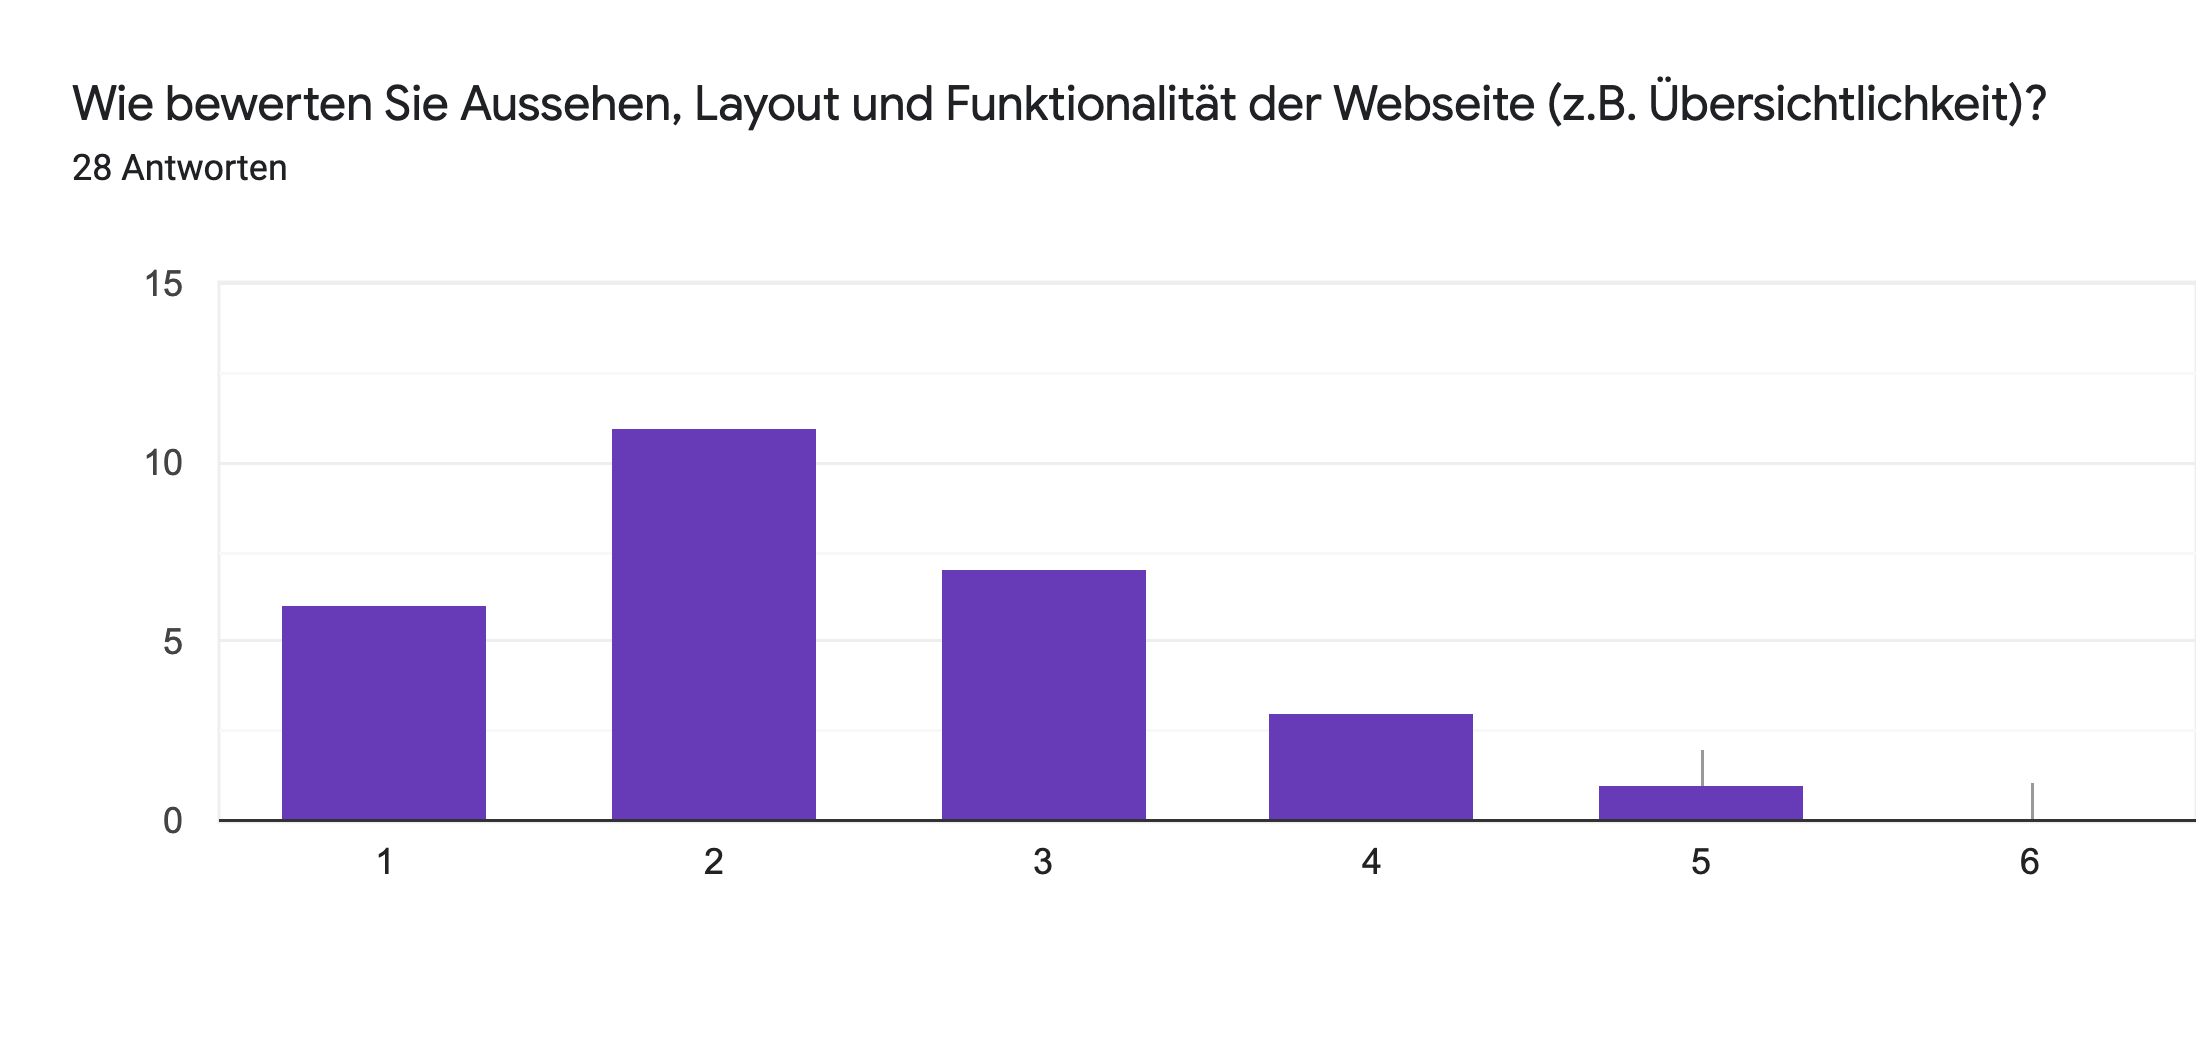
\includegraphics[width=\textwidth]{images/website.png}
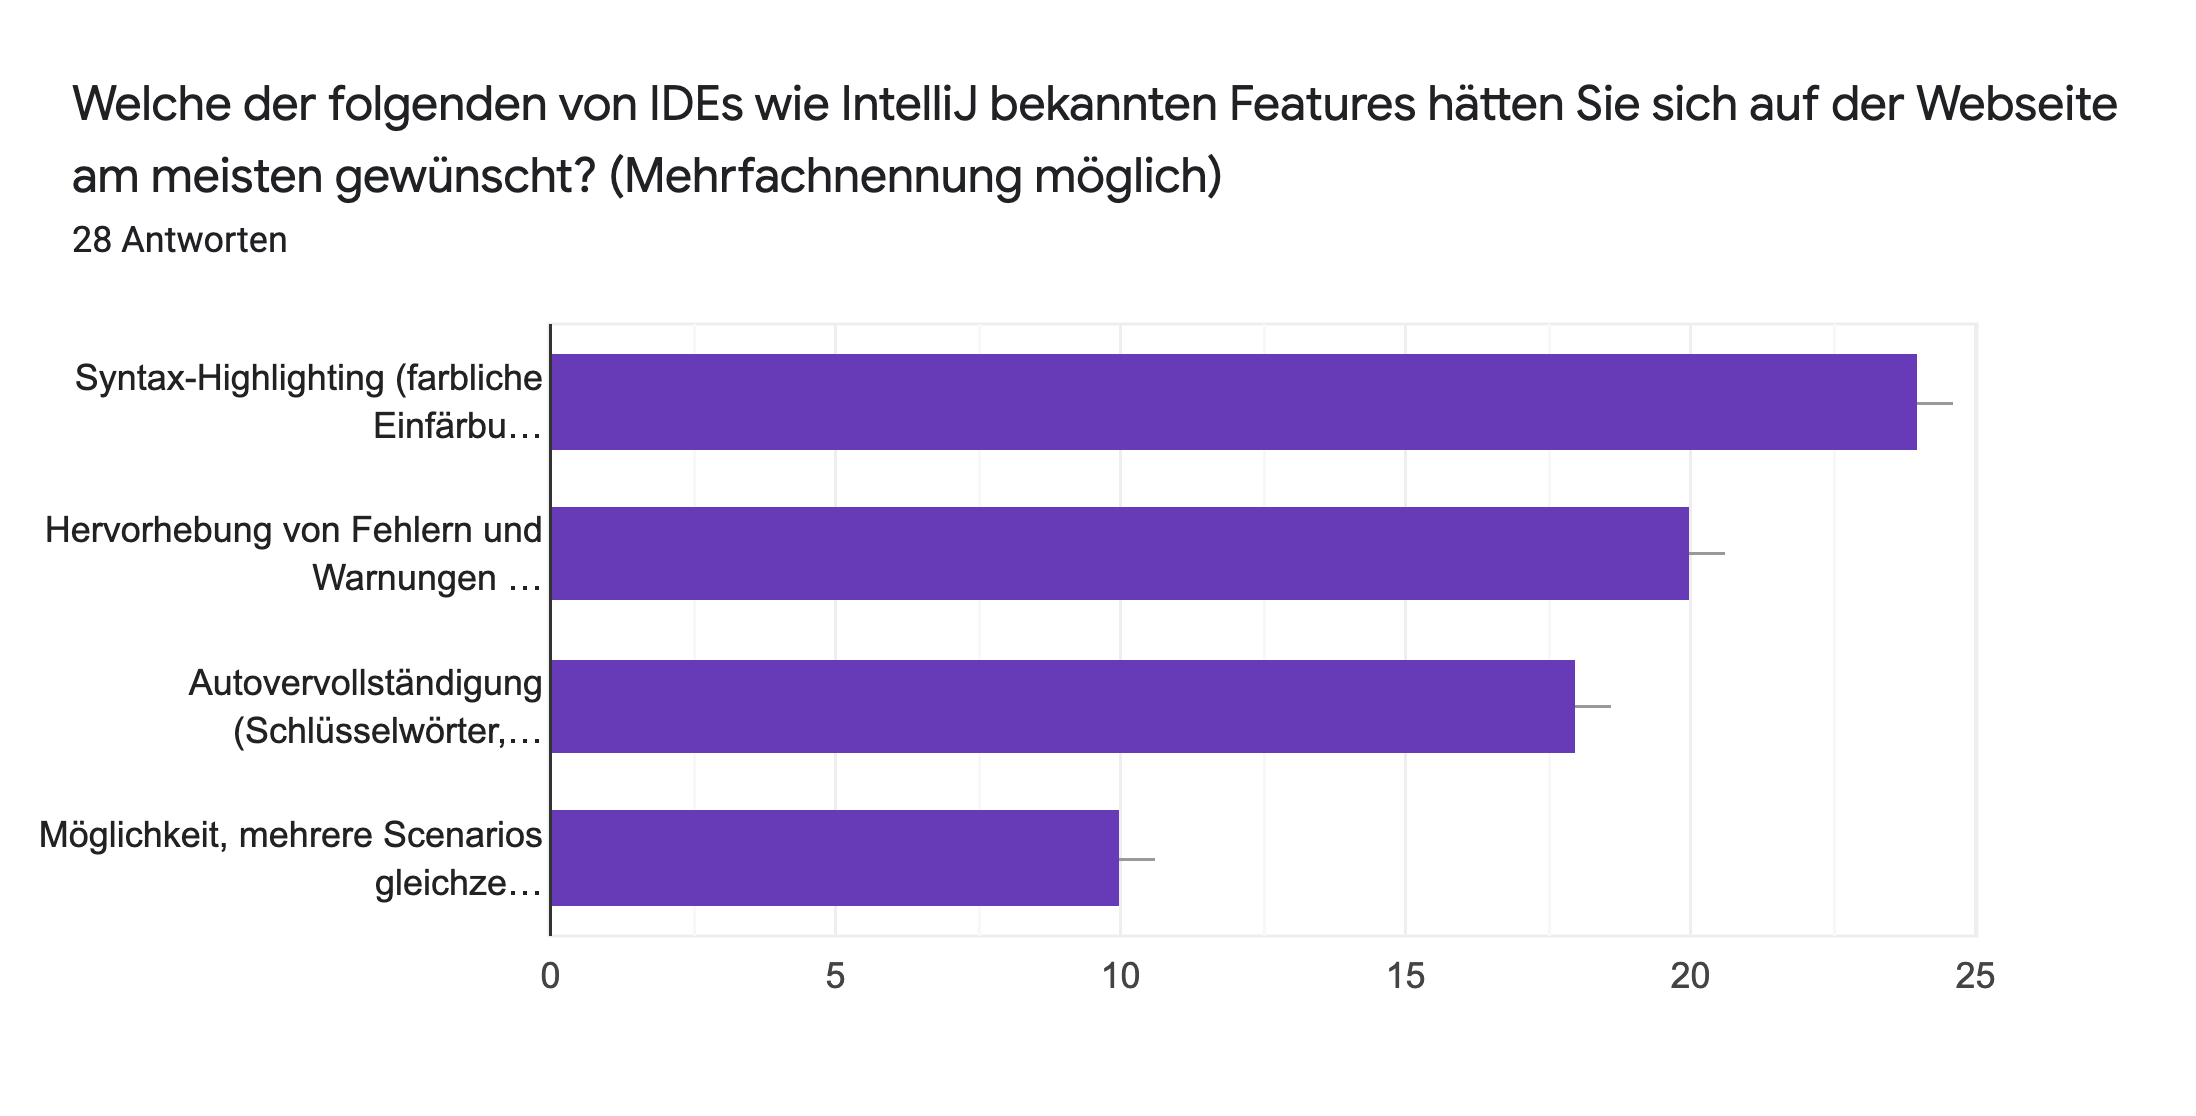
\includegraphics[width=\textwidth]{images/editor-features.png}

%Some guidelines and examples are given in the following.
%
%\section{Figures}
%
%A simple example of a figure can be found in \fig{fig:simple_figure}. A more complex figure including subfigures is show in \fig{fig:figure_with_subfigures}. Here each subfigure can be addressed separately (e.g., \fig{fig:subfigure1} and \fig{fig:subfigure2}). Please use vector graphics (pdf, eps obtained from svg, etc.) whenever possible. Pixel formats like jpeg, bmp, etc. should only be used for real photographs.
%
%\begin{figure}[!h]
%	\centering
%	\fbox{\parbox{5cm}{\centering ~\vspace{1.5cm}\\Dummy\\~\vspace{1.5cm}}} %replace this line by: \includegraphics{path to image}
%	\caption{Simple figure}
%	\label{fig:simple_figure}
%\end{figure}
%
%\begin{figure}[!h]
%	\centering
%	\begin{subfigure}[b]{7cm}
%		\centering
%		\fbox{\parbox{5cm}{\centering ~\vspace{1.5cm}\\Dummy\\~\vspace{1.5cm}}} %replace this line by: \includegraphics{path to image}
%		\caption{Caption of subfigure a (can be empty)}
%		\label{fig:subfigure1}
%	\end{subfigure}
%	\begin{subfigure}[b]{7cm}
%		\centering
%		\fbox{\parbox{5cm}{\centering ~\vspace{1.5cm}\\Dummy\\~\vspace{1.5cm}}} %replace this line by: \includegraphics{path to image}
%		\caption{Caption of subfigure b (can be empty)}
%		\label{fig:subfigure2}
%	\end{subfigure}
%	\caption{Figure using subfigures}
%	\label{fig:figure_with_subfigures}
%\end{figure}
%
%
%\section{Tables}
%
%Examples of tables can be found in \tab{tab:simple_table} and \tab{tab:complex_table}. In general vertical lines are not necessary and should be avoided (see \cite{Fear05} for more about table styles).
%
%\begin{table}[!h]
%	\renewcommand{\arraystretch}{1.1}
%	\caption{A very simple table}
%	\label{tab:simple_table}
%	\centering
%	\begin{tabular}{cccc}
%		\toprule
%		& Apple & Orange & Banana \\
%		\midrule
%		Colour       & green & orange & yellow\\
%		\bottomrule
%	\end{tabular}
%\end{table}
%
%\begin{table}[!h]
%	\renewcommand{\arraystretch}{1.1}
%	\caption{An example of a more complex table}
%	\label{tab:complex_table}
%	\centering
%	\begin{tabular}{ccC{1cm}C{1cm}C{1cm}C{1cm}C{1cm}C{1cm}C{1cm}C{1cm}C{1cm}C{1cm}C{1cm}}
%		\toprule
%		& & \multicolumn{4}{c}{RPAG algorithm} & \multicolumn{5}{c}{RPAGT (proposed)}\\
%		\cmidrule(rl){3-6} \cmidrule(rl){7-11}
%		$N$ & $N_\text{uq}$ & S & add ops & pure reg. & reg. ops & S & add ops & pure reg. & reg. ops & impr.\\
%		\cmidrule(rl){1-11}
%		6   & 3  & 3 & 8  & 1 & 9  & 2 & 5  & 0 & 5  & 44.4\% \\
%		10  & 5  & 3 & 10 & 3 & 13 & 2 & 6  & 2 & 8  & 38.5\% \\
%		13  & 7  & 3 & 14 & 2 & 16 & 2 & 8  & 2 & 10 & 37.5\% \\
%		20  & 10 & 3 & 15 & 4 & 18 & 2 & 9  & 3 & 12 & 33.3\% \\
%		28  & 14 & 3 & 20 & 3 & 23 & 2 & 15 & 2 & 17 & 26.1\% \\
%		41  & 21 & 3 & 31 & 1 & 32 & 2 & 23 & 2 & 25 & 21.9\% \\
%		61  & 31 & 3 & 39 & 3 & 42 & 2 & 32 & 2 & 34 & 19.0\% \\
%		119 & 54 & 3 & 62 & 7 & 69 & 2 & 56 & 1 & 57 & 17.4\% \\
%		151 & 71 & 3 & 79 & 4 & 83 & 2 & 72 & 2 & 74 & 10.8\% \\
%		\cmidrule(rl){1-11}
%		avg.: & 24 & & 30.89 & 3.56 & 33.89 & & 25.11 & 1.78 & 26.89 & 27.7\% \\
%		\bottomrule
%	\end{tabular}
%\end{table}

\end{appendix}

\bibliographystyle{alphadin} %use this for german DIN style
%\bibliographystyle{unsrt} %use this for english texts

\bibliography{thesis}

\end{document}
